\documentclass[10pt]{article}

\usepackage{mathtools, amssymb, bm}
\usepackage{microtype}
\usepackage[utf8]{inputenc}
\usepackage[margin = 1in]{geometry}
\usepackage{booktabs}
\usepackage{graphicx}
\usepackage{xcolor}
\usepackage{tikzsymbols}
\usepackage[hidelinks]{hyperref}
\usepackage{titlesec}

\usepackage{wrapfig}

% \titleformat{\section}{\normalsize\bfseries}{\thesection}{1em}{}
\titleformat{\section}{\large\bfseries}{\thesection}{1em}{}
\setcounter{secnumdepth}{0}

\definecolor{colabcol}{HTML}{960018}
\newcommand{\mycolab}[1]{\textcolor{colabcol}{\textsl{Collaborators:}} #1 \\ }
\newcommand{\mycolaba}[1]{\textcolor{colabcol}{\textsl{Collaborators:}} #1}

\title{
    {\Large Homework 2}
}
\author{
    {\normalsize Aiden Kenny}\\
    {\normalsize STAT GR5204: Statistical Inference}\\
    {\normalsize Columbia University}
}
\date{\normalsize Novermber 26, 2020}

\begin{document}

\maketitle

%' ============================================================================================================================================================
\section{Question 1} \noindent
Suppose that \(Y \sim \mathrm{Bin}(100,p)\), and we want to make an inference about the value of \(p\). We test \(H_0 : p = 0.08\) against \(H_A : p < 0.08\),
and our test \(\delta\) will reject \(H_0\) if and only if \(Y = 6\).
\begin{itemize}
    \item[(a)] The significance \(\alpha\) is the probability of making a Type I error, 
    \begin{align*}
        \alpha(\delta)
        = \mathrm{Pr}(Y = 6 \,|\, p = 0.08)
        = \binom{100}{6} (0.08)^6 (0.92)^{94}
        = 0.123.
    \end{align*}
    \item[(b)] Suppose that \(p = 0.04\). The probability of a Type II error, \(\beta\), is
    \begin{align*}
        \beta(\delta)
        = \mathrm{Pr}(Y \neq 6 \,|\, p = 0.04)
        = 1 - \mathrm{Pr}(Y = 6 \,|\, p = 0.04)
        = 1 - \binom{100}{6} (0.04)^6 (0.96)^{94}
        = 0.895.
    \end{align*}
\end{itemize}

\newcommand{\zgam}{z_{\gamma}}
%' ============================================================================================================================================================
\section{Question 2} \noindent
For a random variable \(Y \sim \mathrm{Binom}(n, p)\), if \(n\) is large enough we can approximate it using a normal distribution with the same mean and 
variance, i.e. \(Y \sim \mathrm{N}(np, np(1-p))\). Then the sample proportion, \(\hat{p} = Y / n\), is also normally distributed as 
\(\hat{p} \sim \mathrm{N}(p, p(1-p)/n)\), and standardizing \(\hat{p}\) gives us \((\hat{p} - p) / \sqrt{p(1-p)/n} \sim \mathrm{N}(0,1)\). 
% maybe put derivation in appendix?
It can then be shown that a \(100\gamma\)\%{} confidence interval for \(\hat{p}\) is given by 
\begin{align*}
    \mathcal{I}
    = \left( ~ 
    \frac{\hat{p} + \zgam^2 / 2n}{1 + \zgam^2 / 2n} - \zgam \cdot \frac{\sqrt{\hat{p}(1 - \hat{p}) / n + \zgam^2 / 4n^2}}{1 + \zgam^2 / n} 
    ~,~ 
    \frac{\hat{p} + \zgam^2 / 2n}{1 + \zgam^2 / 2n} + \zgam \cdot \frac{\sqrt{\hat{p}(1 - \hat{p}) / n + \zgam^2 / 4n^2}}{1 + \zgam^2 / n}
    ~ \right),
\end{align*}
where \(\zgam = \Phi^{-1}((1 + \gamma)/2)\). For this example, we have \(n = 300\) and \(\hat{p} = 75 / 300 = 1/4\), and to get a \(90\)\%{}
confidence interval, we have \(\zgam = 1.645\). Therefore, a \(90\)\%{} confidence interval for \(p\) is \((0.212, 0.294)\).

%' ============================================================================================================================================================
\section{Question 3} \noindent
Suppose we have a random sample \(\bm{X} \overset{\mathrm{iid}}{\sim} \mathrm{Gamma}(4, \beta)\), so \(\mathbb{E}[X_i] = 4\beta\) and \(\mathrm{Var}[X_i] = 4 \beta^2\). The expected 
value and variance of the sample mean \(\bar{X}\) is then given by \(\mathbb{E}[\bar{X}] = 4 \beta\) and \(\mathrm{Var}[\bar{X}] = 4 \beta^2 / n\), and from 
the CLT we have \(\sqrt{n}(\bar{X} - 4 \beta) / 2 \beta = \sqrt{n}(\bar{X} / 2 \beta - 2) \sim \mathrm{N}(0, 1)\). If \(\zgam = \Phi^{-1}((1 + \gamma) / 2)\),
then we have \(\gamma = \mathrm{Pr} (-\zgam \le \sqrt{n}(\bar{X} / 2 \beta - 2) \le \zgam)\). Rearranging to get \(\beta\) in the middle gives us 
\begin{align*}
    \mathcal{I}
    = \left( ~ \frac{2 \bar{X}}{2 + \zgam / \sqrt{n}} ~,~ \frac{2 \bar{X}}{2 - \zgam / \sqrt{n}} ~ \right).
\end{align*}
For this random sample, \(n = 25\), and because we want a \(95.4\)\%{} confidence interval (oddly specific), we have \(\zgam = 2\), so the confidence interval 
is given by \(\mathcal{I} = \big( ~ 5 \bar{X} / 6 ~,~ 5 \bar{X} / 4 ~ \big)\). 

%' ============================================================================================================================================================
\section{Question 4} \noindent
Suppose that \(X \sim \mathrm{Binom}(100, p)\), where \(p \in (1/4, 1/2)\) is unknown. We test \(H_0 : 1/2\) against \(H_A : p = 1/4\) using \(\delta :\) 
reject \(H_0\) if \(X \le 3\). That is, our rejection region is \(\mathcal{S}_X = \{0,1,2,3\}\), and so the power function for this test is 
\begin{align*}
    \pi(p \,|\, \delta)
    = \mathrm{Pr}(X \in \mathcal{S}_X \,|\, p)
    = \sum_{k=0}^3 \binom{10}{k} p^k (1 - p)^{n - k}.
    % = (1 - p)^{10} + 10 p (1 - p)^9 + 45 p^2 (1 - p)^8 + 120 p^3 (1 - p)^7.
\end{align*}

%' ============================================================================================================================================================
\section{Question 5} \noindent
Suppose \(X_1, X_2 \overset{\mathrm{iid}}{\sim} \mathrm{Exp}(1/\theta)\), where \(\theta > 0\), which means \(\mathbb{E}[X_i] = \theta\) and \(\mathrm{Var}[X_i] = \theta^2\). 
The joint density is 
\begin{align*}
    f_{\bm{X}}(\mathbf{x}) 
    = \frac{\mathrm{e}^{-x_1/\theta}}{\theta} \cdot \frac{\mathrm{e}^{-x_2/\theta}}{\theta}
    = \frac{\mathrm{e}^{-(x_1 + x_2)/\theta}}{\theta^2}
    % = \frac{\mathrm{exp}(-(x_1 + x_2)/\theta)}{\theta^2}
\end{align*}
Consider the transformation \(Y_1 = X_1 + X_2\) and \(Y_2 = X_2\), which implies \(Y_1 \sim \mathrm{Gamma}(2, 1/\theta)\) and \(Y_2 \sim \mathrm{Exp}(1/\theta)\).
We note that because \(f_{\bm{X}}(\mathbf{x})\), which is also the likelihood function of the random sample, is a function of \(y_1\) and \(\theta\), so it is
a sufficinet statistic. 
In vector notation, the transformation is given by \(\bm{Y} = \mathbf{A} \bm{X}\), where \(\mathbf{A} = \left[ \begin{smallmatrix}
    1 & 1 \\ 0 & 1
\end{smallmatrix} \right]\), and so \(\bm{X} = \mathbf{A}^{-1}\bm{Y}\), where \(\mathbf{A}^{-1} = \left[ \begin{smallmatrix}
    1 & -1 \\ 0 & 1
\end{smallmatrix} \right]\). Therefore, the joint density of \(Y_1\) and \(Y_2\) is 
\begin{align*}
    g_{\bm{Y}}(\mathbf{y}) 
    = f_{\bm{X}} \big( \mathbf{x} \big) \cdot \left| \,\mathrm{det} \left( \frac{\partial \mathbf{A} \mathbf{x}}{\partial \mathbf{x}} \right) \right|
    = f_{\bm{X}} \big( \mathbf{A}^{-1}\mathbf{y} \big) \cdot \left| \,\mathrm{det} \left( \mathbf{A} \right) \right|
    = \frac{\mathrm{e}^{-(y_1 - y_2 + y_2)/\theta}}{\theta^2} \cdot 1
    = \frac{\mathrm{e}^{-y_1/\theta}}{\theta^2},
\end{align*}
for \(0 < y_2 < y_1\). 
Because \(Y_2 \sim \mathrm{Exp}(1/\theta)\), we have \(\mathbb{E}[Y_2] = \theta\), and so \(Y_2\) is an unbiased estimator for \(\theta\). 
The conditional density of \(Y_2\) given \(Y_1\) is 
\begin{align*}
    g_{Y_2|Y_1}(y_2 \,|\, y_1)
    = \frac{g_{\bm{Y}(\mathbf{y})}}{g_{Y_1}(y_1)}
    = \frac{\mathrm{e}^{-y_1/\theta} / \theta^2}{y_1 \mathrm{e}^{-y_1/\theta}}
    = \frac{1}{y_1},
\end{align*}
and so the conditional expectation of \(Y_2\) given \(Y_1\) is 
\begin{align*}
    \mathbb{E}[Y_2 \,|\, y_1] 
    = \int y_2 \cdot g_{Y_2|Y_1}(y_2 \,|\, y_1) \;\partial y_2
    = \int_0^{y_1} \frac{y_2}{y_1} \;\partial y_2
    = \frac{y_2^2}{2 y_1} \bigg|_0^{y_1}
    = \frac{y_1}{2}
    \coloneqq \varphi(y_1).
\end{align*}
As is standard, we can define the random variable \(\varphi(Y_1)\), and immediately see that \(\mathbb{E}[\varphi(Y_1)] = \mathbb{E}[Y_2] = \theta\). 
In addition, we have 
\begin{align*}
    \mathbb{E}[\varphi(Y_1)^2]
    = \int \varphi(y_1)^2 \cdot g_{Y_1}(y_1) \;\partial y_1
    = \int_0^{\infty} \frac{y_1^2}{4} \cdot \frac{y_1 \mathrm{e}^{- y_1 / \theta}}{\theta^2}
    = \frac{3\theta^2}{2} \int_0^{\infty} \frac{y_1^{4 - 1} \cdot \mathrm{e}^{- y_1 / \theta}}{\theta^4 \Gamma(4)} \;\partial y_1
    = \frac{3\theta^2}{2},
\end{align*}
and so \(\mathrm{Var}[\varphi(Y_1)] = \mathbb{E}[\varphi(Y_1)^2] - \mathbb{E}[\varphi(Y_1)]^2 = \theta^2 / 2\). 

%' ============================================================================================================================================================
\section{Question 6} \noindent
% \begin{wrapfigure}{r}{0.45\textwidth}
%     \centering
%     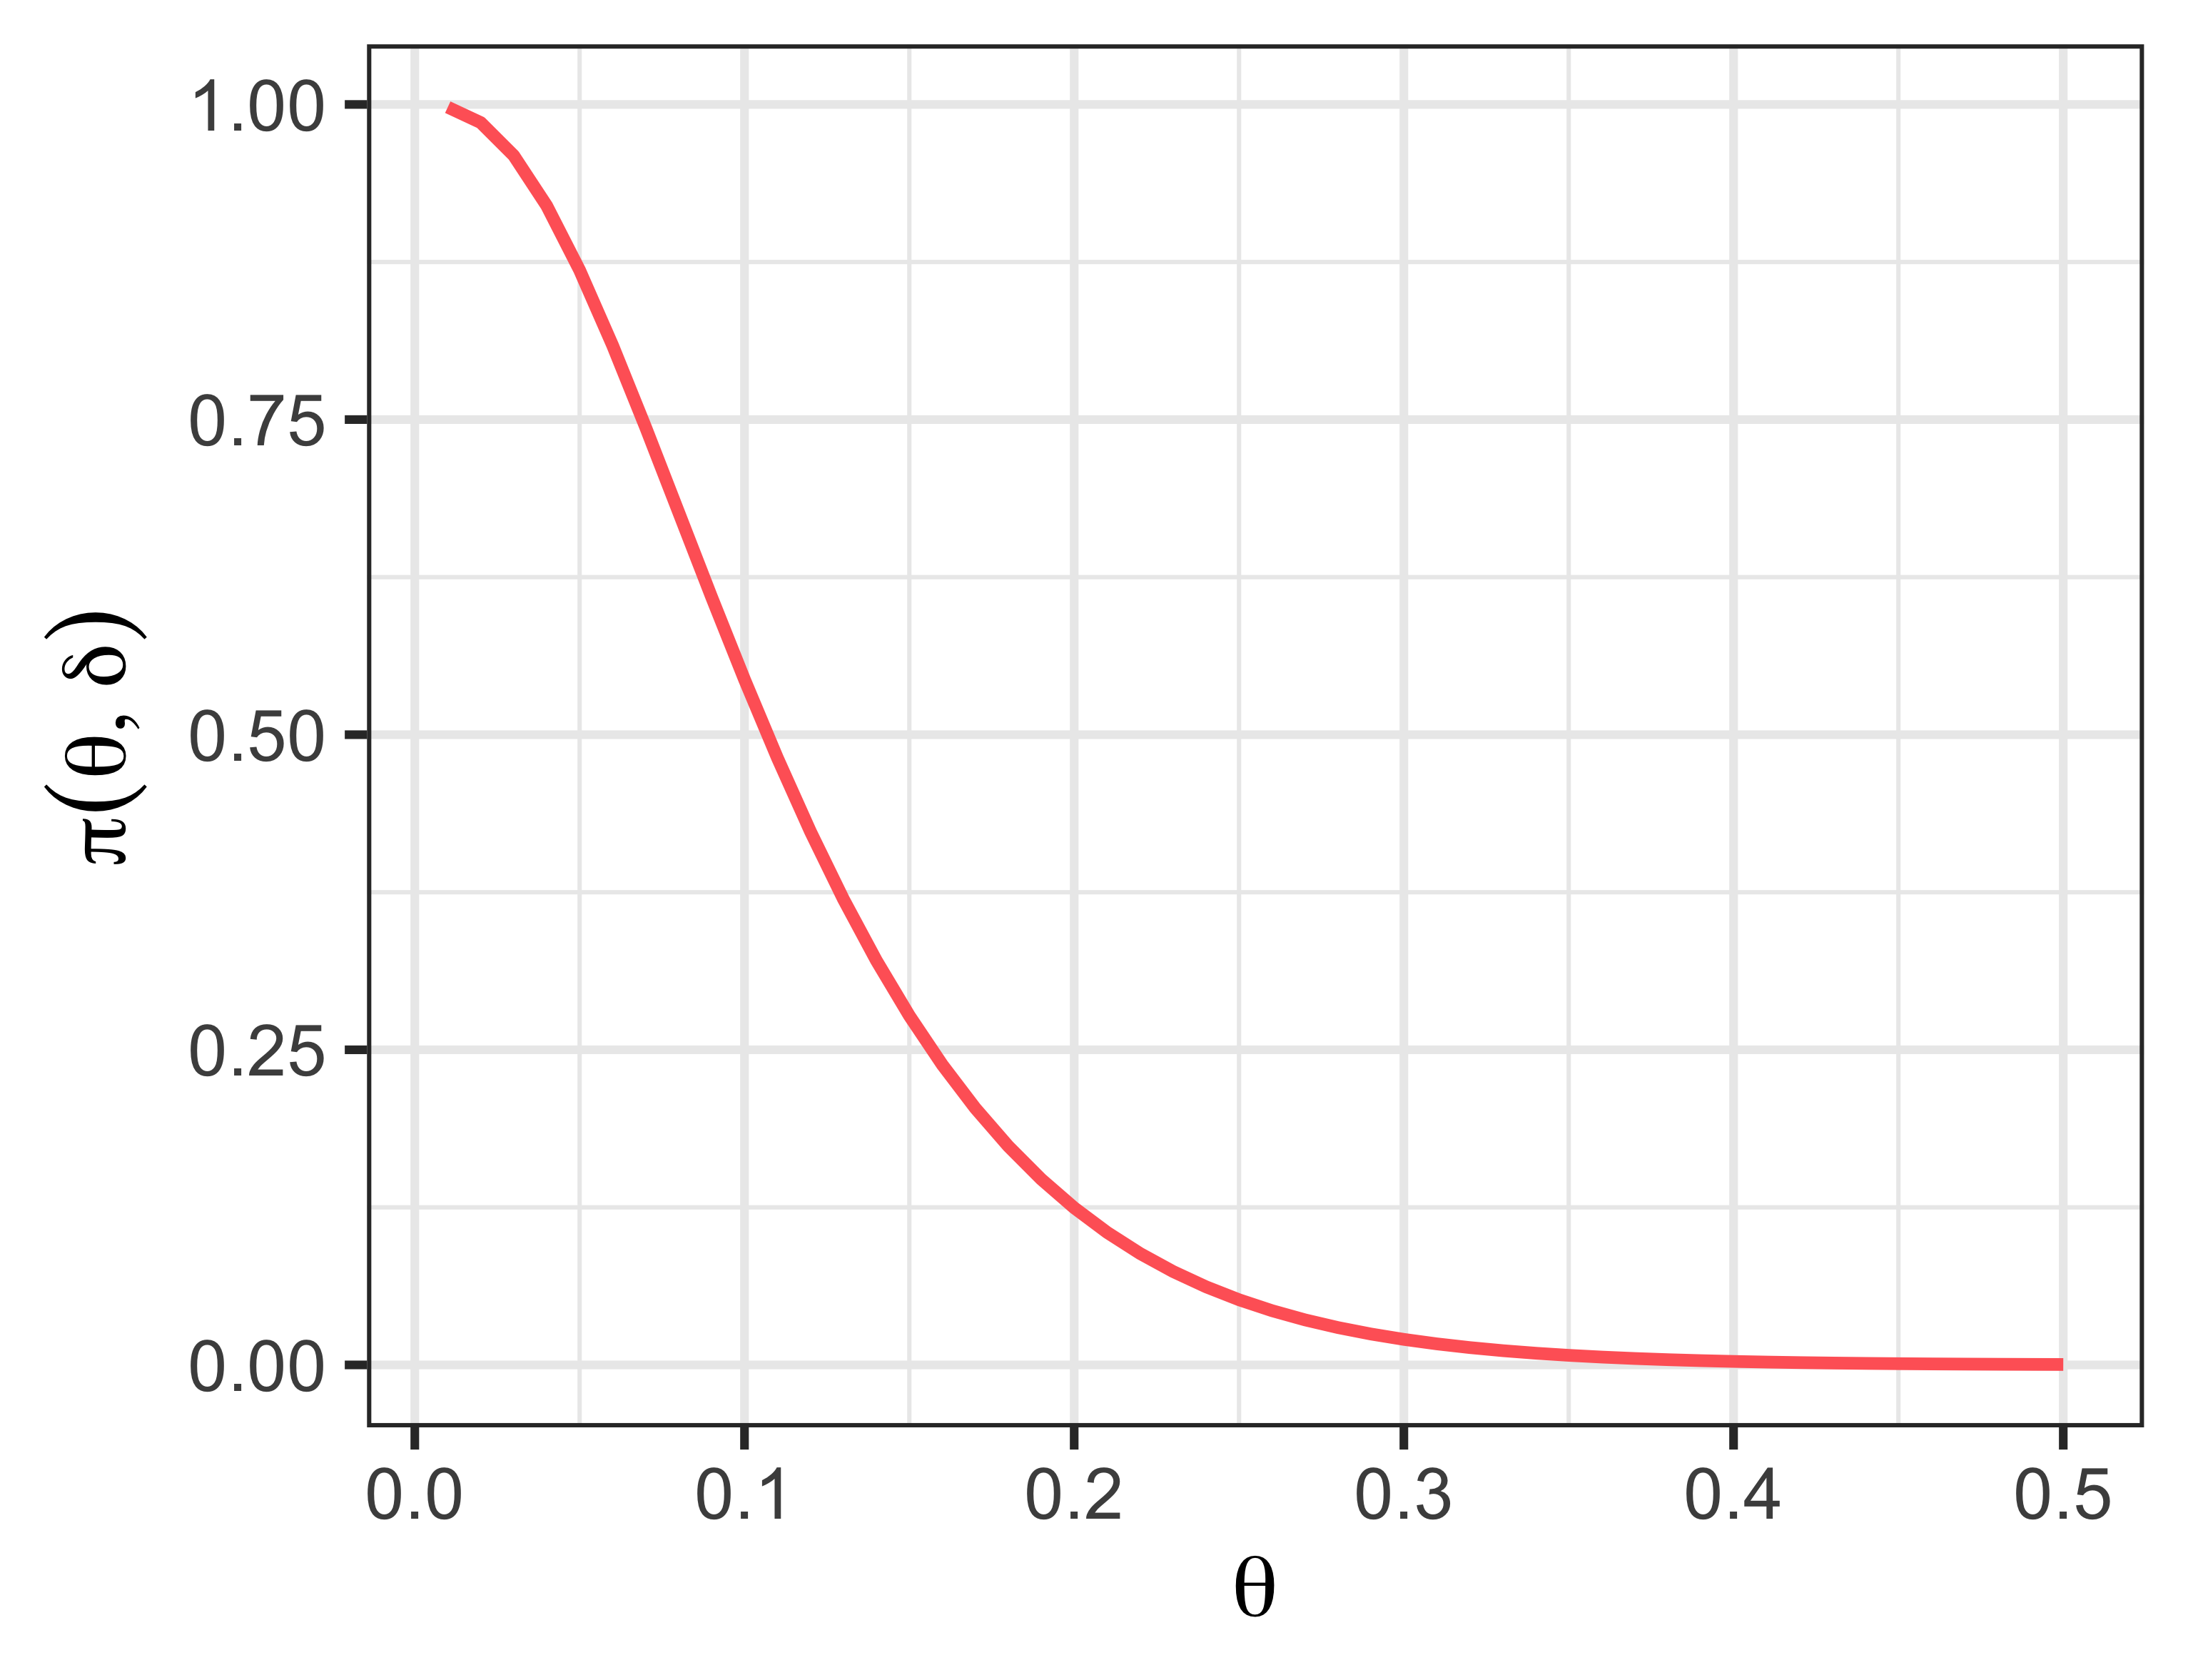
\includegraphics[width = 0.4\textwidth]{img/q06-power-function.png}
%     \caption{The power function \(\pi(\theta \,|\, \delta)\).}
%     \label{q06-power-function}
% \end{wrapfigure}
Suppose that \(\bm{X} \overset{\mathrm{iid}}{\sim} \mathrm{Poisson}( \theta)\). We test \(H_0 : \theta = 1/2\) against \(H_A : \theta < 1/2\) using 
our procedure \(\delta :\) reject \(H_0\) if the test statistic \(Y = \mathbf{1}^T \bm{X} = \sum X_i \le 2\). Since it is a sum of independent Poisson random 
variables, our test statistic is also a Poisson random variable, namely \(Y \sim \mathrm{Poisson}(n \theta)\), and the rejection region for \(Y\) is 
\(\mathcal{S}_Y = \{0,1,2\}\). Therefore, for \(\theta \in (0,1/2]\), the power function of \(\delta\) is given by 
\begin{align*}
    \pi(\theta \,|\, \delta)
    = \mathrm{Pr}(Y \in \mathcal{S}_Y \,|\, \theta)
    = \sum_{k=0}^2 \frac{(n\theta)^k \mathrm{e}^{-n\theta}}{k!}.
\end{align*}
\begin{figure}
    \centering
    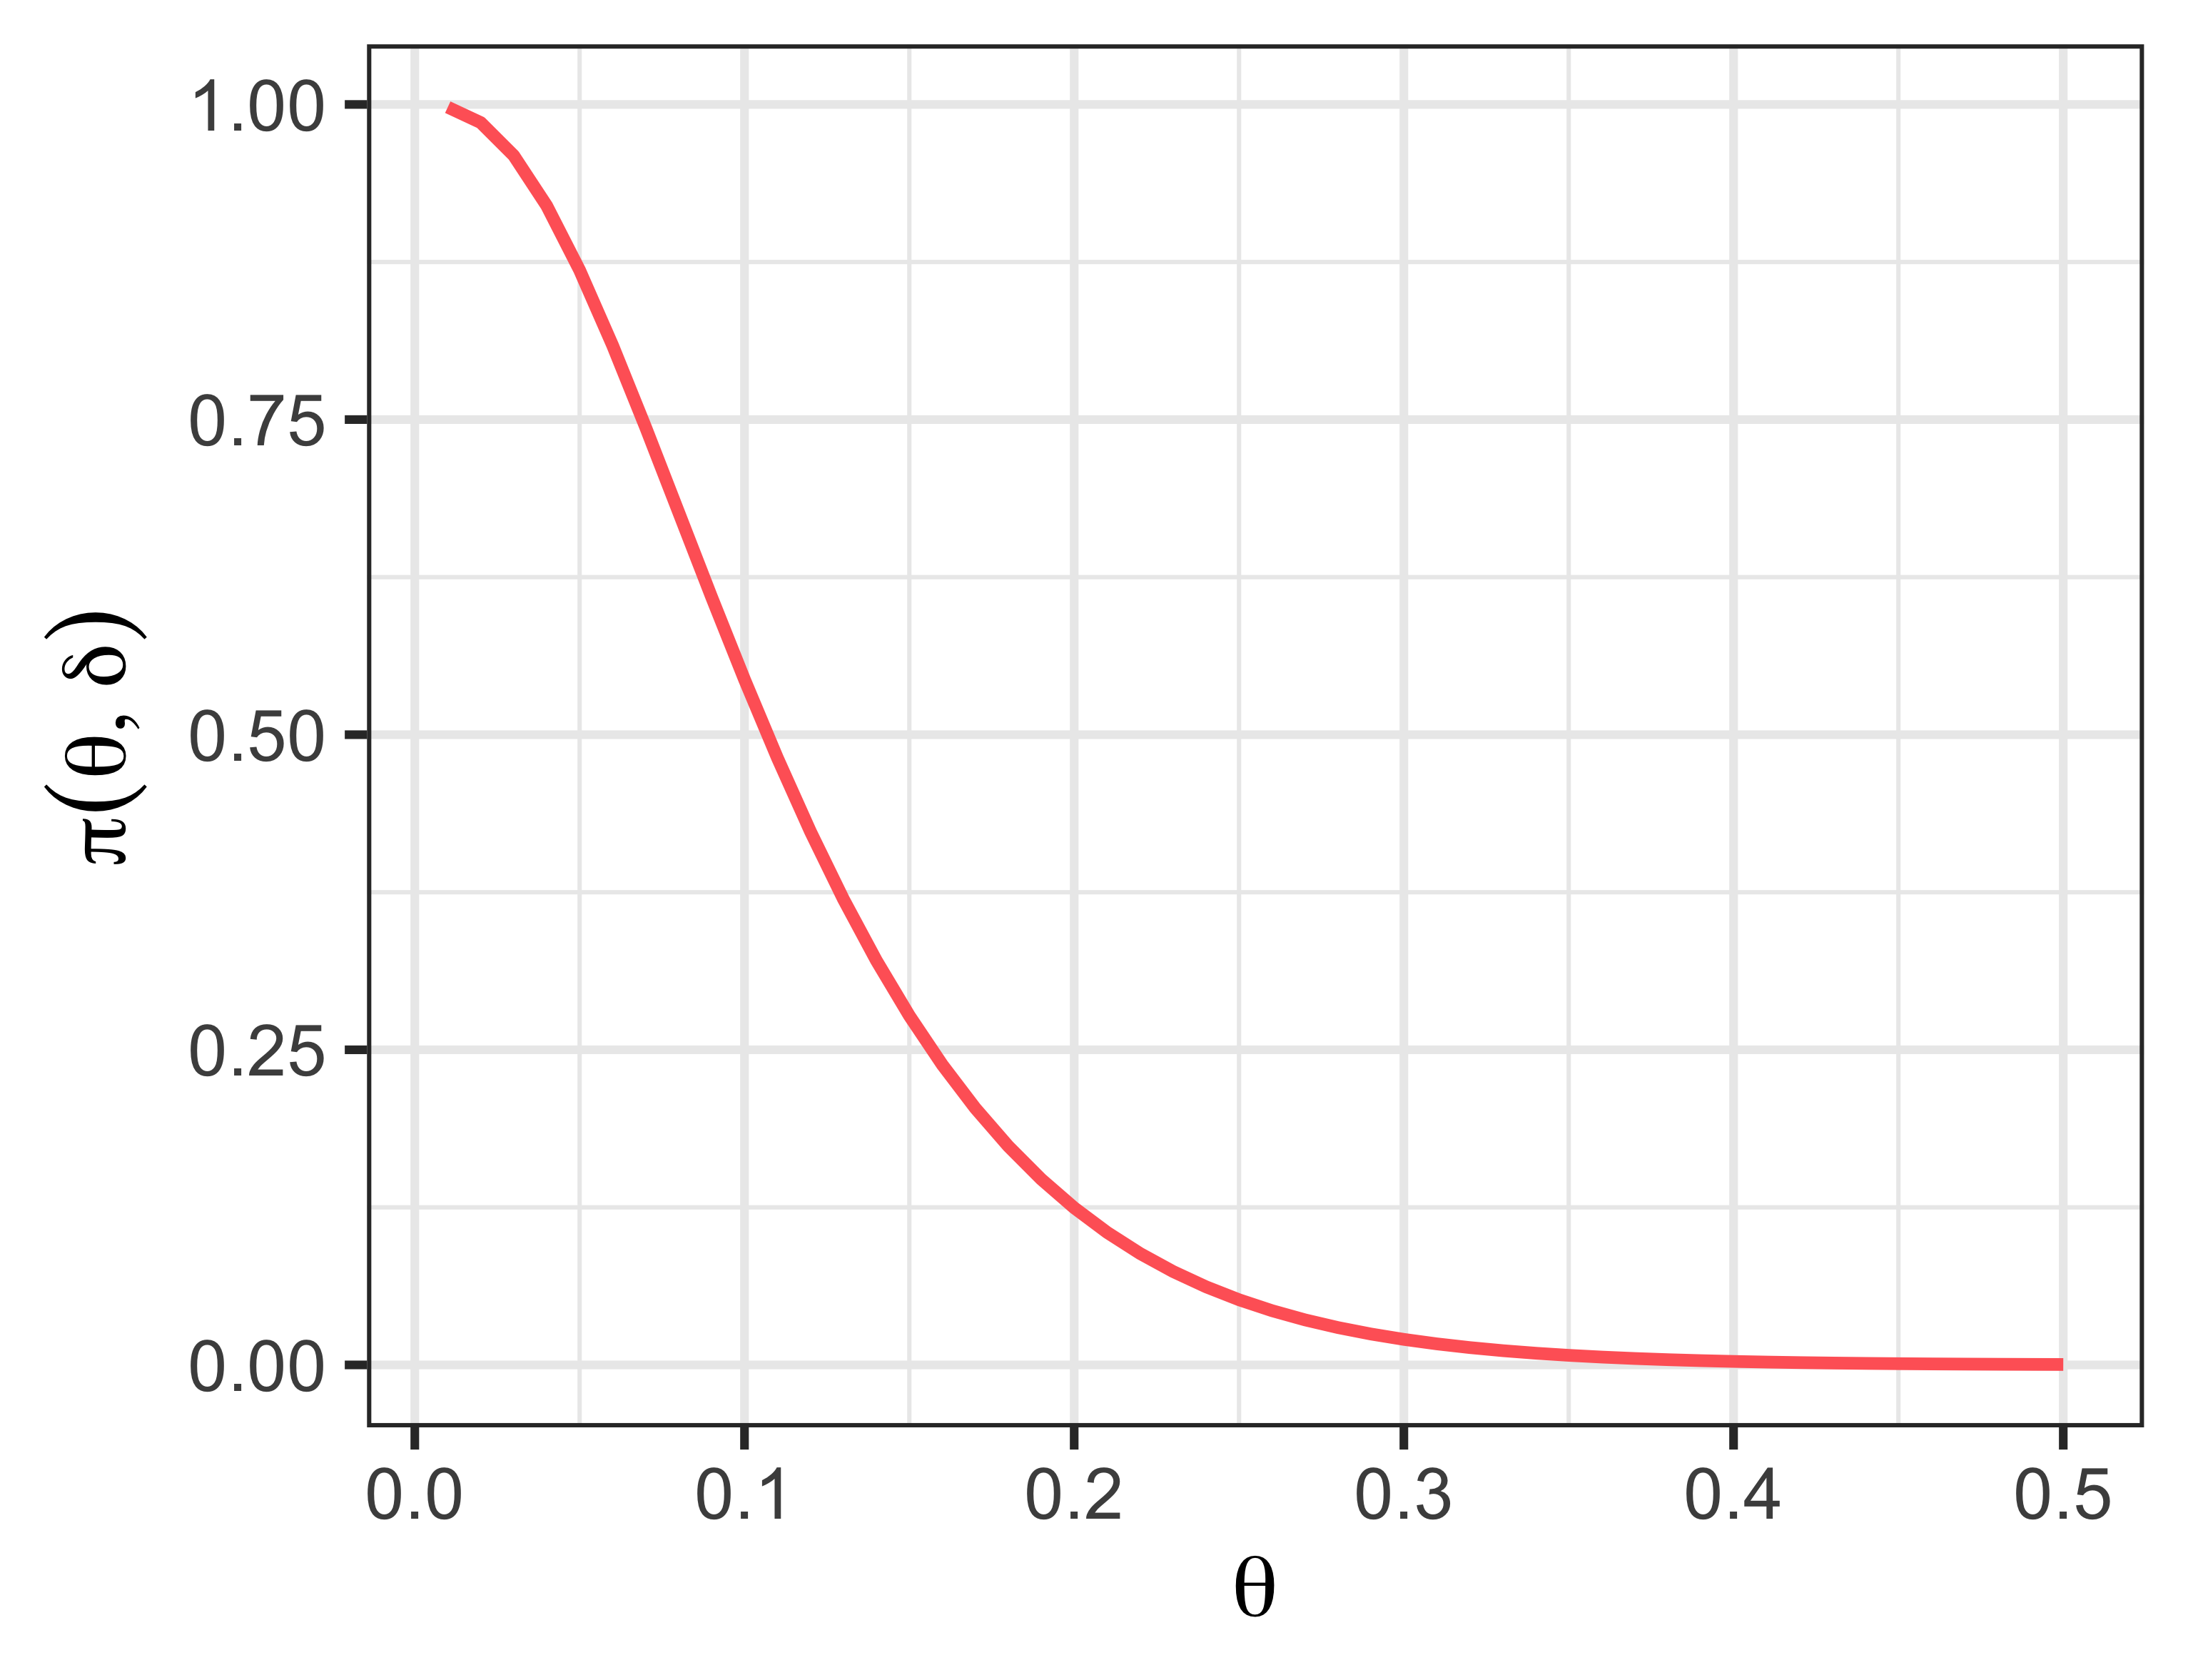
\includegraphics[width = 0.45\textwidth]{img/q06-power-function.png}
    \caption{The power function \(\pi(\theta \,|\, \delta)\).}
    \label{q06-power-function}
\end{figure}
A graph of \(\pi(\theta\,|\,\delta)\) can be found in Figure \ref{q06-power-function}.
% , where we can see the maximum value occurs as \(\theta \to 0\). 
The values of \(\pi(\theta\,|\,\delta)\) when \(\theta = \{1/2,1/3,1/4,1/6,1/12\}\) are given by 
\(0.062, 0.238, 0.423, 0.677, 0.920\), respectively, and have also been marked on Figure \ref{q06-power-function}.
The significance of this test is given by \(\alpha(\delta) = \pi(1/2 \,|\, \delta) = 0.062\).

%' ============================================================================================================================================================
\section{Question 7} \noindent
Let \(X_1, \ldots, X_n \overset{\mathrm{iid}}{\sim} \mathrm{Unif}(0, \theta)\), where \(\theta\) is unknown, and let \(Y_1, \ldots, Y_n\) be the \(n\)
order statistics of the random sample. We are testing \(H_0 : \theta = 1\) against \(H_A : \theta > 1\) with procedure
\(\delta :\) reject \(H_0\) if \(Y_n \ge c\), where \(c\) is an unknown constant that will be determined by the significance of \(\delta\). 
If \(Y_n\) is the \(n\)th order statistic of \(\bm{X}\), its cdf and density are respectively given by \(F_{Y_n}(y_n) = (y_n / \theta)^n\)
and \(f_{Y_n}(y_n) = n y_n^{n-1} / \theta^n\) for \(y_n \in [0, \theta]\). 
\begin{itemize}
    \item[(b)] The rejection region of \(Y_n\) is \(\mathcal{S}_{Y_n} = [c, \theta]\), and so the power function is given by 
    \begin{align*}
        \pi(\theta \,|\, \delta)
        = \mathrm{Pr}(Y_n \in \mathcal{S}_{Y_n} \,|\, \theta)
        = F_{Y_n}(\theta) - F_{Y_n}(c)
        = 1 - \frac{c^n}{\theta^n}.
    \end{align*}
    \item[(a)] To have a significance level of \(\alpha = 0.05\), we must have \(\alpha(\delta) = \pi(1 \,|\, \delta) = 1 - c^n \overset{\mathrm{set}}{=} 0.05\), 
    and solving for \(c\) gives us \(c = \sqrt[n]{0.95}\), and the power function with this level of significance is 
    \(\pi(\theta \,|\, \delta) = 1 - 0.95 / \theta^n\). 
    The question specifically asks for \(n = 4\), in which case \(c = \sqrt[4]{0.95}\) and \(\pi(\theta \,|\, \delta) = 1 - 0.95 / \theta^4\).
    More generally, for any specified significance level \(\alpha_*\), we will have 
    \(c = \sqrt[n]{1 - \alpha_*}\) and \(\pi(\theta \,|\, \delta) = 1 - (1 - \alpha_*) / \theta^n\). 
\end{itemize}

%' ============================================================================================================================================================
\section{Question 8} \noindent
Let \(\bm{X} \overset{\mathrm{iid}}{\sim} \mathrm{N}(\mu, \sigma^2)\), where both \(\mu\) and \(\sigma^2\) are unknown. We want to test 
\(H_0 : \sigma^2 = \sigma^2_0\) against \(H_A : \sigma^2 > \sigma^2_0\) using procedure \(\delta :\) reject \(H_0\) if \(nS^2/\sigma^2_0 \ge c\), where \(c\) 
will be determined by the significance of the test. 
Our test statistic is based off of \(S^2 = \frac{1}{n} \sum_{i=1}^n (X_i - \bar{X})^2\), and we know that \(T(\bm{X}) \coloneqq nS^2 / \sigma^2_0 \sim \chi^2(n-1)\). 
The rejection region for our test statistic is \(\mathcal{S}_{T(\bm{X})} = [c, \infty)\), and we would like to find a value of \(c\) such that the significance
is \(\alpha = 0.025\). 
\begin{align*}
    \alpha(\delta)
    = \pi(\sigma^2_0 \,|\, \delta)
    = \mathrm{Pr} \big( T(\bm{X}) \in \mathcal{S}_{T(\bm{X})} \,|\, \sigma^2_0 \big)
    % = \int_c^{\infty} f(t) \;\partial t
    % = \int_c^{\infty} \frac{1}{2^{\frac{n-1}{2}} \Gamma \left( \frac{n-1}{2} \right)} \cdot t^{\frac{n-3}{2}} \cdot \mathrm{e}^{-t/2} \;\partial t
    % = \int_c^{\infty} \frac{1}{2^{(n-1)/2} \Gamma \left( (n-1)/2 \right)} \cdot t^{(n-3)/2} \cdot \mathrm{e}^{-t/2} \;\partial t
    = \int_c^{\infty} \frac{t^{(n-3)/2} \cdot \mathrm{e}^{-t/2}}{2^{(n-1)/2} \Gamma \left( (n-1)/2 \right)} \;\partial t
    \overset{\mathrm{set}}{=} 0.025.
\end{align*}
There is no way to derive a closed form relationship between \(c\) and \(\alpha\) like we did in question 7, but using \texttt{R} we can write a function 
to find the value of \(c\) for a given significance value \(\alpha\). When \(n = 13\) and \(\alpha = 0.025\), we have \(c = 23.337\). To find a general 
formula of \(\pi(\sigma^2 \,|\, \delta)\), we notice that if \(T(\bm{X}) \ge c\), then \(S^2 \ge c \sigma^2_0 / n\), which serives as a rejection region for 
\(S^2\). Since \(n S^2 / \sigma^2 \sim \chi^2(n-1)\) for any value of \(\sigma^2\), it can be shown that \(S^2 \sim \mathrm{Gamma}\big( (n-1)/2, n / 2 \sigma^2\big)\).
Therefore, the power function is given by 
\begin{align*}
    \pi(\sigma^2 \,|\, \delta)
    = \mathrm{Pr} (S^2 \ge c \sigma^2_0 / n \,|\, \sigma^2)
    = \int_{c\sigma^2_0 / n}^{\infty} \frac{x^{(n - 3)/2} \cdot \mathrm{e}^{- nx/2 \sigma^2}}{\big( n / 2 \sigma^2 \big)^{(n-1)/2} \Gamma \big( (n-1)/2 \big)} \;\partial x,
\end{align*}
where \(c\) is chosen to make \(\alpha(\delta) = 0.025\) (or any specified value, for that matter). Again, there is no closed form solution to this function,
but using \texttt{R} we can find its values, and given a specified value of \(\sigma^2_0\), we will always have \(\pi(\sigma^2_0 \,|\, \delta) = \alpha\)
as desired. 

%' ============================================================================================================================================================
\section{Question 9} \noindent
If \(\bm{X} \overset{\mathrm{iid}}{\sim} \mathrm{N}(\mu, \sigma^2)\) with unknown \(\mu\) and \(\sigma^2\), then a \(\gamma\)\%{} confidence interval
for \(\mu\) is given by 
\begin{align*}
    \mathcal{I} = \Big( ~\bar{X} - t_{\gamma}(n) \cdot S / \sqrt{n} ~,~ \bar{X} + t_{\gamma}(n) \cdot S / \sqrt{n} ~ \Big),
\end{align*}
where \(t_{\gamma}(n) = T_{n-1}^{-1} ( (1 + \gamma) / 2 )\) is the \((1 + \gamma) / 2\)th quantile of the \(t\) distribution with \(\mathrm{df} = n-1\) and \(S\)
is the sample standard deviation. 
The length of this confidence interval is given by 
\begin{align*}
    \Delta 
    % = \bar{X} + T_{n-1}^{-1}\big( (1 + \gamma) / 2 \big) \frac{S}{\sqrt{n}} - \bigg( \bar{X} - T_{n-1}^{-1}\big( (1 + \gamma) / 2 \big) \frac{S}{\sqrt{n}} \bigg)
    = \max (\mathcal{I}) - \min (\mathcal{I})
    = \Big( \bar{X} + t_{\gamma}(n) \cdot S / \sqrt{n} \Big) - \Big( \bar{X} - t_{\gamma}(n) \cdot S / \sqrt{n} \Big)
    = 2 t_{\gamma}(n) \cdot S / \sqrt{n}.
\end{align*}
The squared length is then given by \(\Delta^2 = 4 t_{\gamma}^2(n) \cdot S^2 / n\). 
Because the sample variance is an unbiased estimator for \(\sigma^2\), we have \(\mathbb{E}[\Delta^2] = \mathbb{E} \big[ 4 t_{\gamma}^2(n) \cdot S^2 / n \big] = 4 t_{\gamma}^2(n) \cdot \sigma^2 / n\).
We now set \(\mathbb{E}[\Delta^2] < \sigma^2 / 2\), and after some cancellations, we see that we need \(t_{\gamma}^2(n) / n < 1/8\). There is no way to find a
closed-form expression for this, so we will have to check the value of \(t_{\gamma}^2(n) / n\) for increasing values of \(n\). I set up a \texttt{while} 
loop in \texttt{R} to solve for it, and when \(\gamma = 0.9\), we find that \(n = 24\) is the smallest value of \(n\) such that \(\mathbb{E}[\Delta^2] < \sigma^2 / 2\).

%' ============================================================================================================================================================
\section{Question 10} \noindent
Let \(\bm{X} \overset{\mathrm{iid}}{\sim} \mathrm{N}(\theta, \sigma^2)\), where \(\theta\) is unknown and \(\sigma^2\) is known, and we assume prior that 
\(\theta \sim \mathrm{N}(\mu, \nu^2)\), where both \(\mu\) and \(\nu^2\) are known. 
\begin{itemize}
    \item[(a)] Since normal distributions are are conjugate to normal sampling, it follows
    that \(\theta \,|\, \mathbf{x} \sim \mathrm{N}(\tilde{\mu}, \tilde{\sigma}^2)\), where 
    \begin{align*}
        \tilde{\mu}
        = \frac{\sigma^2 \mu + n \nu^2 \bar{x}}{\sigma^2 n \nu^2}
        ~~~\text{and}~~~
        \tilde{\sigma}^2
        = \frac{\sigma^2 \nu^2}{\sigma^2 + n \mu^2}.
    \end{align*}
    We also know that \((\theta \,|\, \mathbf{x} - \tilde{\mu}) / \tilde{\sigma} \sim \mathrm{N}(0,1)\), and so a \(95\)\%{} confidence interval for 
    \(\theta \,|\, \mathbf{x}\) is given by 
    \begin{align*}
        \mathcal{I}
        = \Big( ~ \tilde{\mu} - \Phi^{-1}(0.975) \cdot \tilde{\sigma} ~,~ \tilde{\mu} + \Phi^{-1}(0.975) \cdot \tilde{\sigma} ~ \Big).
        % = \Big( ~ \frac{\sigma^2 \mu + n \nu^2 \bar{x}}{\sigma^2 n \nu^2} - \Phi^{-1}(0.975) \cdot \frac{\sigma^2 \nu^2}{\sigma^2 + n \mu^2} ~,~ \frac{\sigma^2 \mu + n \nu^2 \bar{x}}{\sigma^2 n \nu^2} + \Phi^{-1}(0.975) \cdot \frac{\sigma^2 \nu^2}{\sigma^2 + n \mu^2} ~ \Big)
    \end{align*} 
    \item[(b)] We can think of our interval \(\mathcal{I}\) as a function of \(\nu^2\). To examine what happens to \(\mathcal{I}(\nu^2)\) as \(\nu^2 \to \infty\), we 
    will first look at \(\tilde{\mu}\) and \(\tilde{\sigma}\). Using L'Hopital's rule, we have
    \begin{align*}
        \lim_{\nu^2 \to \infty} \tilde{\mu}
        &= \lim_{\nu^2 \to \infty} \frac{\sigma^2 \mu + n \nu^2 \bar{x}}{\sigma^2 n \nu^2}
        = \lim_{\nu^2 \to \infty} \frac{n \bar{x}}{n}
        = \bar{x}, \\
        \lim_{\nu^2 \to \infty} \tilde{\sigma}
        &= \lim_{\nu^2 \to \infty} \sqrt{\frac{\sigma^2 \nu^2}{\sigma^2 + n \mu^2}}
        = \sqrt{ \lim_{\nu^2 \to \infty} \frac{\sigma^2 \nu^2}{\sigma^2 + n \mu^2}}
        = \sqrt{ \lim_{\nu^2 \to \infty} \frac{\sigma^2}{n}}
        % = \sqrt{\frac{\sigma^2}{n}}
        = \frac{\sigma}{\sqrt{n}},
    \end{align*}
    and so \(\mathcal{I}(\nu^2) \to \big( ~\bar{x} - \Phi^{-1}(0.975) \cdot \sigma / \sqrt{n} ~,~ \bar{x} + \Phi^{-1}(0.975) \cdot \sigma / \sqrt{n} ~ \big)\),
    which is a \(95\)\%{} confidence interval for \(\theta\). 
\end{itemize}

%' ============================================================================================================================================================
\section{Question 11} \noindent
Let \(\bm{X} \overset{\mathrm{iid}}{\sim} \mathrm{Unif}(0, \theta)\), where \(\theta\) is unknown, and let \(Y = X_{(n)}\) be the \(n\)th order statistic. 
\begin{itemize}
    \item[(a)] Let \(F_i(x) = \mathrm{Pr}(X_i \le x) = x / \theta\) for all \(i \in \{1, \ldots, n\}\). Then the cdf of \(Y\) is 
    \(G(y) = \prod_{i = 1}^n F_i(y) = \left( y / \theta \right)^n\), since all of the \(X_i\)'s are independent. The density of \(Y\) is then given by 
    \(g(y) = n y^{n - 1} / \theta^n\) for \(y \in [0, \theta]\). By letting \(W = Y / \theta\), we have \(Y = \theta W\) and \(\partial Y / \partial W = \theta\), 
    so the density of \(Y / \theta\) is given by \(h(w) = g\big( y(w) \big) \cdot \theta = n w^{n-1}\) for \(w \in [0,1]\). The cdf is then seen to be 
    \(H(w) = w^n\), and so the quantile is given by \(H^{-1}(w) = \sqrt[n]{w}\).
    % \begin{align*}
    %     G(y) 
    %     = \mathrm{Pr}(Y \le y)
    %     = \mathrm{Pr} \big( X_1 \le y \cap \cdots \cap X_n \le y \big)
    %     = \prod_{i = 1}^n F_i(y) = \left( \frac{y}{\theta} \right)^n
    % \end{align*}
    \item[(b)] Since we must have \(y \le \theta\), it is natural that \(Y\) will underestimate \(\theta\), and is therefore biased. We have 
    \begin{align*}
        \mathbb{E}[Y]
        = \int_{0}^{\theta} y \cdot \frac{n y^{n-1}}{\theta^n} \,\partial y
        = \frac{n}{\theta^n} \int_0^{\theta} y^n \,\partial y
        = \frac{n}{\theta^n} \cdot \frac{y^{n+1}}{n+1} \bigg|_{0}^{\theta}
        = \frac{n}{\theta^n} \cdot \frac{\theta^{n+1}}{n+1}
        % = \frac{n}{n+1} \cdot \theta,
        = \frac{n\theta}{n+1},
    \end{align*}
    and so the bias is \(\mathrm{bias}(Y) = \mathbb{E}[Y] - \theta = -\theta / (n+1)\). 
    \item[(d)] Using the cdf of \(Y / \theta\), for any interval involving \(Y / \theta\), we have \(\mathrm{Pr}(a \le Y / \theta \le b) = b^n - a^n\), where 
    \(a, b \in (0, 1]\). Rearranging the terms inside the interval gives us \(\mathrm{Pr}(Y / b \le \theta \le Y / a) = b^2 - a^2 \overset{\mathrm{set}}{=} \gamma\).
    That is, as long as we impose the constraint that \(b^2 - a^2 = \gamma\), any interval \((Y/b, Y/a)\) is a \(\gamma\)\%{} confidence interval for \(\theta\). 
\end{itemize}

%' ============================================================================================================================================================
\section{Question 12} \noindent
Suppose that \(X \sim \mathrm{P}\), where \(\mathrm{P}\) is an unknown distribution, and we want to test \(H_0: \mathrm{P} = \mathrm{Unif}(0,1)\) against 
\(H_1: \mathrm{P} = \mathrm{N}(0, 1)\). The densities of both distributions (within their support) are given by \(f_0(x) = 1\) for \(x \in [0,1]\) and 
\(f_2(x) = (2\pi)^{-1/2}\mathrm{exp}(-x^2 / 2)\), respectively, and so our test statistics is 

%Determine the most powerful test of size 0.01, and calculate the power of the test when H1 is true.

\end{document}